\section{Embedded System}
\subsection*{Hardware}
\begin{frame}
\frametitle{ReWac Board Hardware}
    \begin{columns}
        \column{0.6\textwidth}
        \begin{figure}
        \centering
        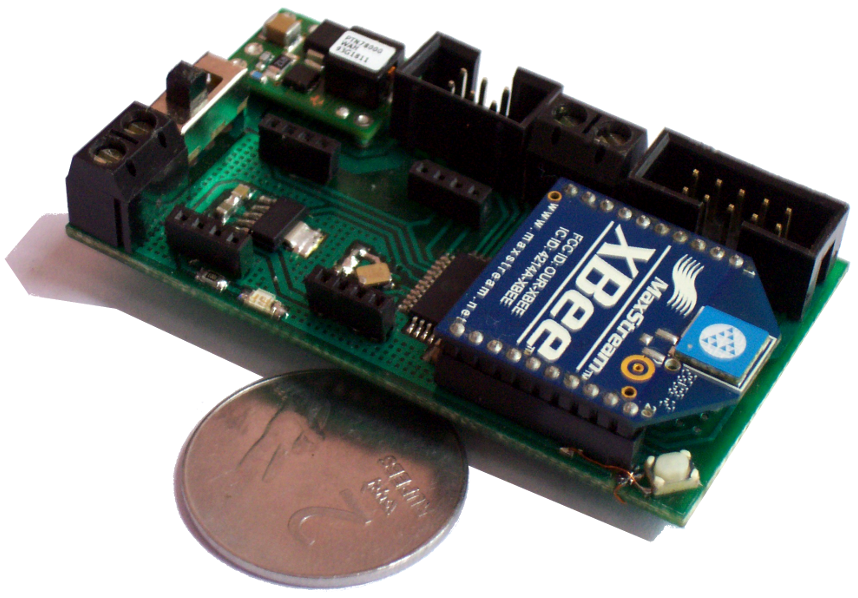
\includegraphics[scale=0.2]{fig/rewac.png}
        \end{figure}
        
        \column{0.4\textwidth}
        \begin{itemize}
        \item
        Microchip dsPIC33F\\[0.05in]
        16 bit, 40 MIPS\\[0.1in]
        \item
        Accelerometer\\[0.05in]
        2.162 LSB/mg\\[0.1in]
        \item
        Gyroscope (50 Hz)\\[0.05in]
        0.07326 $^o/s/$LSB\\[0.1in]
        \item
        5A motor driver\\[0.1in]
        \item
        XBee module\\[0.1in]
        \end{itemize}
    \end{columns}
\end{frame}

\subsection*{Kalman Filter}
\begin{frame}
\frametitle{Kalman Filter}
\begin{block}{Why}
\begin{itemize}
\item
Pitch attitude estimate
\item
Computing power
\end{itemize}
\end{block}

\begin{block}{How}
\begin{equation*}
\bm{x} = [x_1\;\;x_2]^T = [\theta\;\;\dot{\theta}]^T
\end{equation*}
\vspace{0.075in}
\begin{equation*}
\bm{x}_{k+1} = \bm{A}\:\bm{x}_k + \bm{B}\:\bm{u}_k + \bm{w}_k
\end{equation*}
\vspace{0.075in}
\begin{equation*}
y_{k+1} = \bm{C}\:\bm{x}_{k+1} + z_{k+1}
\end{equation*}
\end{block}

\begin{block}{Tricks}
\begin{itemize}
\item
\alert{Sparse covariance matrix}
\item
Remove matrix operations
\item
\alert{Fixed point arithmetic}
\end{itemize}
\end{block}
\end{frame}

\begin{frame}
\frametitle{Attitude Estimation}

\begin{columns}

\column{0.5\textwidth}

\begin{block}{Accelerometer}
\begin{itemize}
\item
Slow, absolute reading
\item
\alert{Body accelerations} - Noise
\item
High frequency noise
\end{itemize}
\end{block}

\begin{block}{Gyroscope}
\begin{itemize}
\item
Fast
\item
Drifts slowly, randomly
\end{itemize}
\end{block}

\column{0.5\textwidth}
\begin{itemize}
    \item
    After liftoff $\sim$ { \greencol 250 ms}\\[0.1in]
    \begin{itemize}
        \item
        Only force is gravity\\[0.1in]
        \item
        Both sensors used\\[0.2in]
    \end{itemize}

    \item
    Free fall $\sim$ {\greencol 250 ms}\\[0.1in]
    \begin{itemize}
        \item
        No accelerometer reading\\[0.1in]
        \item
        Propagate using rate only\\[0.2in]
    \end{itemize}

    \item
    Stance $\sim$ {\greencol 150 ms}\\[0.1in]
    \begin{itemize}
        \item
        \alert{Ankle potentiometer}
    \end{itemize}

\end{itemize}
\end{columns}
\end{frame}

\begin{frame}
\frametitle{High Frequency Input sampled at 50 Hz}
\begin{figure}
\centering
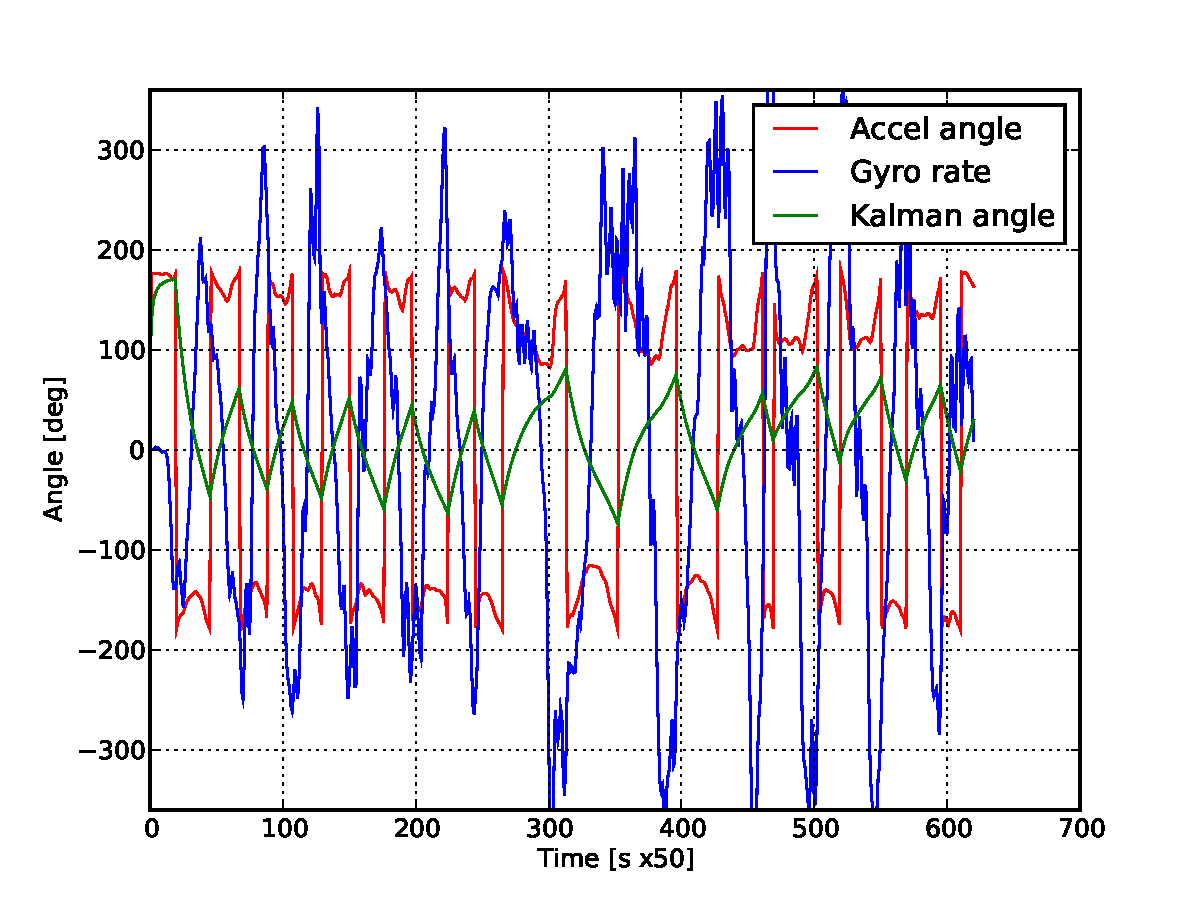
\includegraphics[width=\textwidth]{fig/kf.pdf}
\end{figure}
\end{frame}
